\documentclass{article}
\usepackage{tikz}

\begin{document}

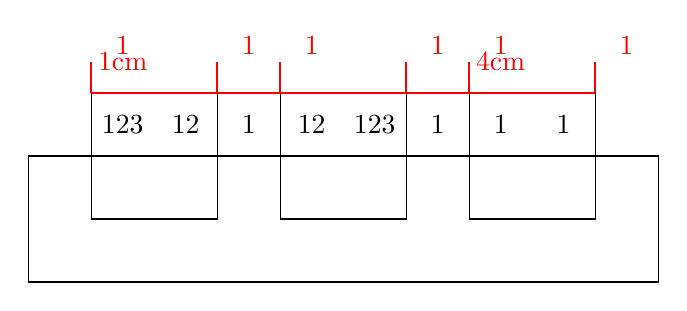
\begin{tikzpicture}[scale=0.8]
    % Draw the main rectangle
    \draw (0,0) rectangle (10,2);
    
    % Draw the inner rectangles
    \draw (1,1) rectangle (3,3);
    \draw (4,1) rectangle (6,3);
    \draw (7,1) rectangle (9,3);
    
    % Label the inner rectangles
    \node at (1.5,2.5) {123};
    \node at (2.5,2.5) {12};
    \node at (3.5,2.5) {1};
    \node at (4.5,2.5) {12};
    \node at (5.5,2.5) {123};
    \node at (6.5,2.5) {1};
    \node at (7.5,2.5) {1};
    \node at (8.5,2.5) {1};
    
    % Draw the horizontal line with labels
    \draw[red, thick] (1,3) -- (9,3);
    \node[red] at (1.5,3.5) {1cm};
    \node[red] at (7.5,3.5) {4cm};
    
    % Draw the vertical lines
    \draw[red, thick] (1,3) -- (1,3.5);
    \draw[red, thick] (3,3) -- (3,3.5);
    \draw[red, thick] (4,3) -- (4,3.5);
    \draw[red, thick] (6,3) -- (6,3.5);
    \draw[red, thick] (7,3) -- (7,3.5);
    \draw[red, thick] (9,3) -- (9,3.5);
    
    % Draw the vertical lines with labels
    \node[red] at (1.5,3.75) {1};
    \node[red] at (3.5,3.75) {1};
    \node[red] at (4.5,3.75) {1};
    \node[red] at (6.5,3.75) {1};
    \node[red] at (7.5,3.75) {1};
    \node[red] at (9.5,3.75) {1};
\end{tikzpicture}

\end{document}